\documentclass[12pt]{article}
\usepackage[utf8]{inputenc}
\usepackage{graphicx}
\usepackage{titlepic}
\usepackage{caption}
\usepackage{subcaption}
\usepackage[a4paper, total={6in, 8in}]{geometry}

% \documentclass{beamer}
\usepackage{amsmath}

\newcommand{\namesigdate}[2][5cm]{%
  \begin{tabular}{@{}p{#1}@{}}
    #2 \\[0.4\normalbaselineskip] \hrule \\[0pt]
    {\small } \\[2\normalbaselineskip] 
  \end{tabular}
}

\title{\vspace*{\fill} \textbf{Video Description using Deep Learning}
	  \\ {\large \textbf{Summer Undergraduate Research Award}}
	  \\  \vspace{3mm} 
\includegraphics[width=5cm]{logo.jpg}}

\author{
	\textbf{Suyash Agrawal}\\ 
	2015CS10262\\
	Computer Science\\
	CGPA: 9.87 \\
	Mob: 9717060183\\
	cs1150262@iitd.ac.in
	\and
	\textbf{Madhur Singhal}\\ 
	2015CS10235\\
	Computer Science\\
	CGPA: 8.66\\
	Mob: 9540972599\\
	cs1150235@iitd.ac.in
}
\date{\textbf{Supervisor:-} \\ \textbf{Subhashis Banerjee} \\ Professor \\ Department of CSE \\ suban@cse.iitd.ac.in\\ IIT Delhi\\
\vspace*{\fill}}




\begin{document}
	\maketitle

\begin{center}
\noindent\rule{3.2cm}{0.4pt} 
\end{center}

% \begin{flushright}
% \noindent\rule{3.2cm}{0.4pt} 
% \\ \textbf{Prof. S. Arun Kumar}
% \\ Head of Department
% \\ Department of CSE
% \\ sak@cse.iitd.ernet.in
% \end{flushright}
	\newpage

	\section{Introduction}
		\textit{\textbf{Video Description}} is the process of discovering knowledge, structures, patterns and events of interest in video data and generating a description of them in natural human language. Video Description is an open problem in computer vision and currently the predominant source of video description is manual human work. 
		\newline
		Video Description has wide variety of applications. It can help visually impaired people ``see'' the world by describing the scene around them. It has also use in automated surveillance by analyzing the videos in real time and reporting malicious or unusual activities. It can also be used to efficiently index large video databases based upon their content for ease of accessibility.

		\begin{figure}[ht!]
		\centering
		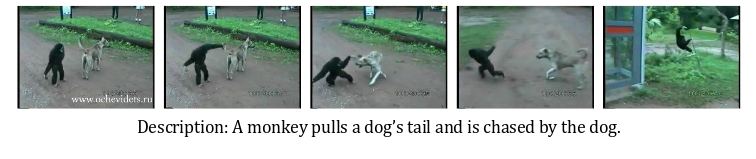
\includegraphics[width=1.0\textwidth]{description.png}
		\caption{Sample Video Description\label{fig0}}
		\end{figure}		
In this project we created an end to end Neural Network pipeline which generates an english sentence from a given input video clip. This pipeline is inspired by the recent success of Convolutional Neural Networks in image analysis and that of Sequence to Sequence Recurrent Neural Networks in Machine Translation. Our network can be thought of as translating between a video clip and an english sentence, wherein individual frames of the video are ``words'' in the video language. Since our network is end to end we have a combined loss function for the whole network based on the sentence returned by the network and the desired sentence. Finally we use an Adam Optimizer and backpropagation through the network to optimize the weights. In practice the Convolutional Neural Networks are too big to be trained using the limited video clip datasets we have and thus we use a CNN that has already been trained on the separate task of image classification for which there is a huge dataset called Imagenet.

	\section{Past Work}

		Much of the prior work in this field is focused on generating natural language descriptions from images. Recently the use of an end to end deep neural network architecture which takes an image as input and generates an english description has  been shown to give excellent results. We extended this approach to a Video Description network which takes in a sequence of frames as input and generates an english description of the actions happening in the video. For this we use an encoder-decoder framework widely used in Machine Translation, which maps a variable length input to a variable length output. 

	\section{Data}
The data used is a crucial factor in the effectiveness of a complex neural network like ours. We primarily used the following two datasets for training and validation purposes.
	\begin{enumerate}
		\item
			\textbf{Microsoft Research - Video to Text (MSR-VTT)}: The dataset contains 41.2 hours and 200K clip-sentence pairs in total, covering the most comprehensive categories and diverse visual content, and representing the largest dataset in terms of sentence and vocabulary.
		\item
			\textbf{Montreal Video Annotation Dataset (M-VAD)}: The M-VAD movie description corpus is another recent collection of about 49,000 short video clips from 92 movies. It is similar to MPII-MD, but only contains AD data and only provides automatic alignment.
		\end{enumerate}
		Both of these datasets consist of short Youtube video clips (average length near 20 seconds) and english sentences (average length near 12 words) describing the clips. Most of the video clips also have a synchronized audio clip which we utilize in some of our experiments. 
		Empirically we found out that these datasets were big enough for our network to learn proper English language sentence structure and grammar automatically, and the sentences we return are almost always gramatically correct. The datasets also identify a wide host of objects and actions which make the network applicable in general situations.\\
		The main problem we faced with these datasets was that they were not properly sampled and thus there was an inherent bias towards the types of videos seen on Youtube as opposed to those encountered in the real world. For example, the datasets had a large amount of videos of video games which often involve rapidly changing frames and our network began to associate things like car crashes to video game clips. 
\section{Methods}
\subsection{Overall Approach}
	Our approach to video description was motivated by the recent successful approach of using Encoder-Decoder system in Image Description.
	Our pipeline consisted of a CNN network that extracted feateures from the individual video frames, one LSTM network which encoded these features into a fixed length feature vector and another LSTM network which decoded the feature vector into a natural language description.

\subsection{Word Embeddings}
To generate sentences we need a vocabulary, we use a vocabulary which consists of about 13000 words as well as punctuation marks. We also add two special tokens $\langle$Start$\rangle$ and $\langle$End$\rangle$ to the vocabulary to represent the beggining and end of a sentence. Since a simple one-hot representation of a word is very sparse and unstructured, we use a fully connected layer (called the ``embedding layer'' to convert a word to a dense vector space. We experimented with different embedding methods, including random initialization of a trainable embedding layer and using pretrained GloVe or Word2Vec embeddings. Empirically we found out that using pretrained embeddings gives almost identical results to randomly initializing the embedding layer and training it within our pipeline.\\
At the output stage we need another matrix to decode the outputs to words and we used another fully connected layer which gives an output of length vocabulary size with each element representing the probability of that word being generated. Note that while it may seem reasonable to use the same weights in the embedding and decoding layers as first sight, such an approach gives poor results in our experiments since the vector space of embedding outputs and the vector space of decoding inputs are different and unrelated to each other.

\subsection{Video Feature Extraction}

	We used Convolutional neural networks for extracting features from video frames. In recent times CNNs have shown amazing results in object
	detection in images and thus they form a natural choice in extracting features from images. Also, since videos are a sequences of images, we
	downsample video frames at a fixed frame rate and then individually extract features from each video frame and concantenate them to get 
	the feature vector of the video.\\
	We used Inception V4 net as our choice of CNN for video feature extraction as it has shown the best results in ImageNet challenge and is thus
	more likely to give better feature extraction from image frames. We also experimented with audio features in the video. Specifially we looked
	at the MFCC features of the audio and we processed these features along with image features in our encoder network to get better representation
	of the video. But we later abandoned this approach as it did not show any significant improvement in the results and also added audio dependency
	to our network which would have made this un-usable in the case of video surveillance and other areas where audio is not available.
	
\subsection{Video Feature Encoding}
	We used a LSTM based network for encoding feature vectors of individual video frames into a single feature vector for the whole clip. This approach is largely inspired by similar approach in machine translation which also use LSTMs for encoding decoding between languages. Here we used the feature
	vector of video frames as inputs to LSTM units and the final hidden state of the LSTM network as the video encoding.\\ 
	We experimented with various types of encoding networks like:
	\begin{itemize}
		\item Single layer LSTM network
		\item Multi layered LSTM network (2-5 layers)
		\item Residual Network Multi Layered LSTM network
		\item Encoder network with Attention Model
	\end{itemize}
	Apart from the above, we also experimented with dropout in between layers and also experimented with audio features concatenated with
	video features.
\subsection{Decoding to Natural Language}
The previous stage gives us a fixed length feature vector which represents the whole video clip. We use this feature vector as the initial hidden state of our decoder LSTM network. After this we feed words (embedded in a vector space as described above) one by one into the LSTM, which gives the next word. There is a special $\langle$Start$\rangle$ token which represents the beginning of a sentence and is always the first one to be given as input. The ouput word is deduced from the output of the LSTM network using a fully connected layer with softmax activation, which results in a vector of length equal to the size of our vocabulary and where each element can be interpreted as the probability of that word coming next in the sentence.\\
Initially we used a greedy approach to sentence formation by taking the word with maximum probability at the output of  each step, adding it to our sentence and feeding it as input in the next step. This approach often resulted in convoluted and inaccurate sentences, since some degree of look-ahead is needed for proper sentence structure. Finally we used \textbf{Beam Search Decoder} to provide us with a  certain amount of look-ahead, and observed our sentences and results both improve dramatically. A Beam Search is a compromise between the totally greedy approach which can be short-sighted and the breadth-first search approach which is not computationally tractable. Instead of choosing the best setence at the end of each step, here we keep a  `beam' of sentences (three sentences in the beam were used in practice). At each step, for each sentence in the beam we consider the top three predictions for the next word and make nine sentences out of those, then we filter down from these nine sentences to three sentences on the basis of the combined probability for the original sentence and the added word.

\subsection{Training Phase}
In traning phase, we had video-caption pairs in our dataset. Using this we first encoded the video into sequence of feature
vectors and after encoding these frames using encoder network we pass the hidden state into the decoder lstm. In this we first
pass the start token $\langle$Start$\rangle$ with the hidden state corresponding to the last encoder lstm unit. The 
decoder lstm unit gave the probability of each word in our vocabulary being the next word in a vector of the size 
of our vocab. At each step we fed the next from correct description into the lstm unit and recorded its output.
Our loss is the sum of the negative log likelihood of the correct word at each step as follows:
$$
	L(V,S) = - \sum_{t=1}^{N}{\log{p_t(S_t)}}
$$
Where,\\
$V$ = Input Video\\
$S$ = Correct caption of video $V$. It is a sequence of words $(S_0,S_1,\ldots,S_N)$\\
$L(V,S)$ = Loss corresponding to video caption pair (V,S)\\
$p_t(S_t)$ = Probability of word $S_t$ in the output of LSTM unit at time $t$.\\\\
The above loss is minimized w.r.t. all the parameters of the Encoder LSTM unit, Decoder LSTM unit,
the top layer of the image embedder CNN and word embeddings.

\subsection{Inference Phase}
We used multiple approaches for inference phase for generating a sentence given a video.
\\The first one was \textbf{Sampling} where we just sample the first word according to p1, then provide the corresponding embedding
as input and sample p2, continuing like this until we sample
the special end-of-sentence token $\langle$End$\rangle$ or some maximum length.
\\The second one is \textbf{BeamSearch}: iteratively consider the set of the k best sentences up to time t as candidates to generate
sentences of size t + 1, and keep only the resulting best k
of them.
We used the BeamSearch approach in the following experiments,
with a beam of size upto 10. Using a beam size of 1 (i.e.,
greedy search) did degrade our results.


\subsection{Dealing with Overfitting}

The main problem we had to deal with throughout the project was overfitting. This is a phenomenon where the Neural Network becomes attuned to the training data itself, rather than learning patterns that can generalize easily to new inputs. This is akin to a student memorizing answers to questions from a guide book and not being able to answer new questions easily. A characteristic indication of overfitting is that the training loss is much less than the validation loss. The main factor influencing overfitting is the \textit{complexity} of the model which is basically the number of trainable parameters in the model and the training method employed. A neural network which is too complex for the problem it is designed to solve will utilize the remaining degrees of freedom to provide lower loss in response to specific training data samples. Also if the network is trained too long or with a poorly designed optimizer it may become specific to training data.\\

To deal with overfitting we experimented a lot and found the following approaches to be very useful. 
\begin{enumerate}
\item \textbf{Adjusting Complexity :} Reducing our LSTM encoder decoder network from a four layer network to a two layer network was very helpful in reducing overfitting. We also reduced the number of parameters is the fully connected layers by reducing the word embedding size.  
\item \textbf{Dropout :} Dropout layers take a vector as input and reuturn a vector where each element is either zero with a certain probability or the original value. Dropout helps with overfitting because even  when the same input is fed multiple times into the network the parameters influencing the output may be different each time. We used a Droput Wrapper on our LSTM cells which makes a certain fraction (we used 0.4) of the LSTM ouputs zero and found that it reduced overfitting.
\item \textbf{Proper Training :} The choice of optimizer is important and thus we decided to use Adam Optimizer which maintains a separate learning rate for each parameter of the model and keeps reducing the rate with time. This keeps the parameters from oscillating wildly and helps with overfitting. We also took care to train the model only as far as it reduced the validation loss and stop when the validation loss started to increase which indicates overfitting.

\end{enumerate}


With all these implemented, ovefitting was a much smaller problem then before and our training loss was mostly near our validation loss.
\subsection{Other experiments}


				\begin{figure}[ht!]
				\centering
					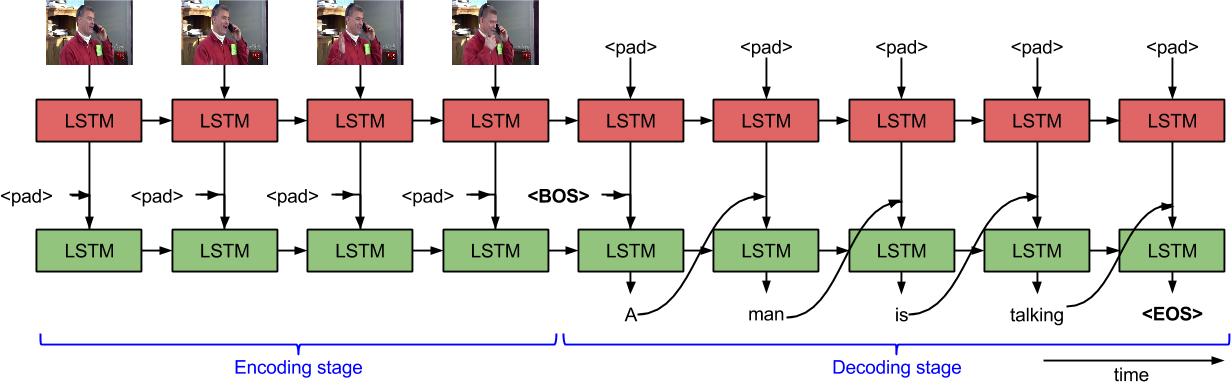
\includegraphics[width=10cm]{s2vt.png}
					\caption{Video description model with 2 LSTM levels\label{fig1}}
				\end{figure}

\section{Results}

\section{Summary}
	

	\section{Uses and applications}
			\begin{itemize}
				\item
					Assisting visually impaired people to get description of their surroundings, thus enabling them to ``see''.
				\item
					Very useful for automated surveillance and theft detection by being able to analyze large amounts of data which is unfeasible to be done by humans.
				\item
					Allowing content based video retrieval by describing the contents of video in textual format which is indexable by web crawlers.
				\item
					This can also be used to detect catastrophic events through security cameras like fire breakout, murder etc.
				\item
					This project can also be applied in helping robotic vision as this project basically allows one to understand what is happening in the video and thus robots will be able to get a ``true'' sense of their surroundings.
			\end{itemize}



	\section{Background} 
			\subsection{Deep Learning}
				Deep Learning is a branch of machine learning in which multiple parameter based models are used in series. In a deep network, there are many layers between the input and output, allowing the algorithm to be executed in multiple processing steps, composed of \textbf{multiple linear and non-linear transformations}. At each layer, the signal is transformed by a processing unit, like an artificial neuron, whose parameters are \textbf{`learned'} through training. Deep Learning has been shown to excel in tasks where the goal is to find \textbf{intuitive} patterns in the data.\cite{deep} In particular, in the field of Computer Vision, deep networks are increasingly used to extract \textbf{feature descriptions and inter-relationships between features} from images.\cite{cs231n}
				\begin{figure}[ht!]
					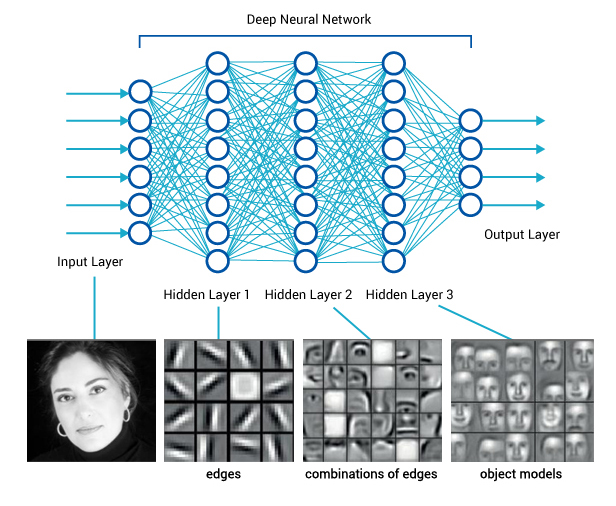
\includegraphics[width=14cm]{blog_deeplearning3.jpg}
					\caption{Illustration of Deep Learning as applied to Vision\label{fig2}}
				\end{figure}	

			\subsection{Convolutional Neural Networks}
			Convolutional Neural Networks (CNN, or ConvNet) are a type of feed-forward artificial neural network in which the connectivity pattern between the neurons is inspired by the organization of the animal visual cortex. Individual cortical neurons respond to stimuli in a restricted region of space known as the \textbf{receptive field}. The receptive fields of different neurons partially overlap such that they tile the visual field. The response of an individual neuron to stimuli within its receptive field can be approximated mathematically by a \textbf{convolution operation}. A Convolutional Neural Network consists of the following layers.\cite{showandtell}
								
				\begin{figure}[ht!]
					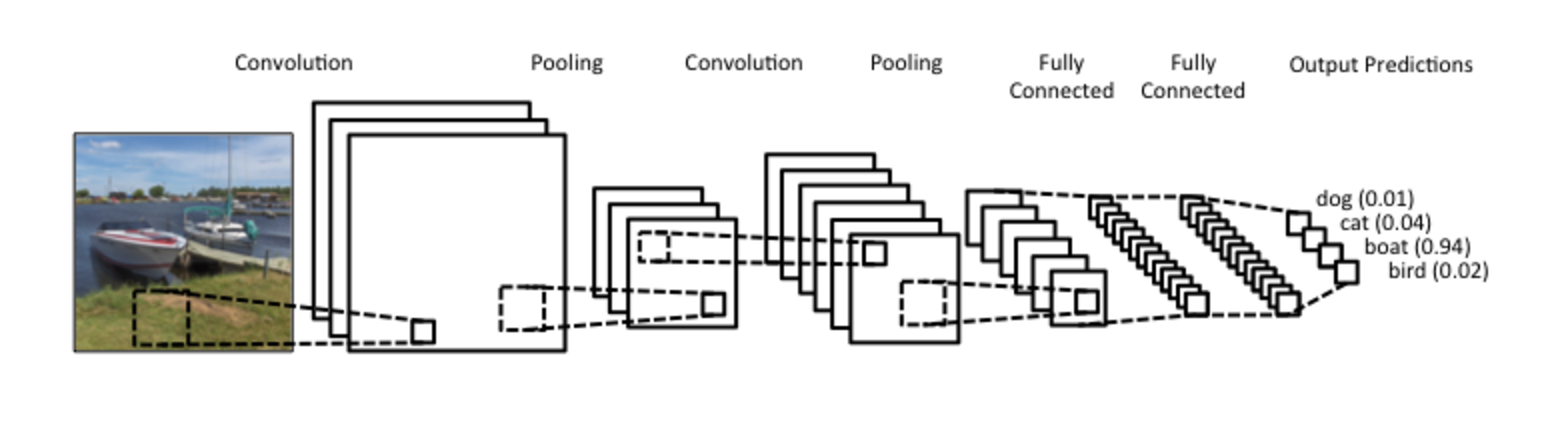
\includegraphics[width=1.0\textwidth]{conv.png}
					\caption{A Typical Convolutional Neural Network\label{fig4}}
				\end{figure}
			%skipping Relu layer since its not in picture assume it to be in conv layer
				\subsubsection{Convolutional Layer}
					The convolution layer is the core building block of a CNN. The layer's parameters consist of a set of \textbf{learnable filters} (or kernels), which have a small receptive field, but extend through the full depth of the input volume. During the forward pass, each filter is convolved across the width and height of the input volume, computing the dot product between the entries of the filter and the input and producing a $2$-dimensional activation map of that filter.\cite{cs231n} As a result, the network learns filters that activate when it detects some specific type of feature at some spatial position in the input.

				\subsubsection{Max Pooling Layer}
					It is common to periodically insert a Pooling layer in-between successive Conv layers in a ConvNet architecture. Its function is to \textbf{progressively reduce the spatial size} of the representation to reduce the amount of parameters and computation in the network, and hence to also control over-fitting. The Pooling Layer operates independently on every depth slice of the input and resizes it spatially, using the max operation.\cite{cs231n}
				\subsubsection{Fully-Connected Layer}
					Finally, after several convolutional and max pooling layers, the high-level reasoning in the neural network is done via fully connected layers. Neurons in a fully connected layer have \textbf{full connections to all activations} in the previous layer, as seen in regular Neural Networks. Their activations can hence be computed with a matrix multiplication followed by a bias offset.\cite{fullyconnected} Thus output of the fully connected layer is a vector with elements representing the `probability' (not in a strictly statistical sense) of the image containing specific objects or actions.

			\subsection{Long Short Term Memory Networks}
			    \begin{figure}[ht!]
			    	\centering
					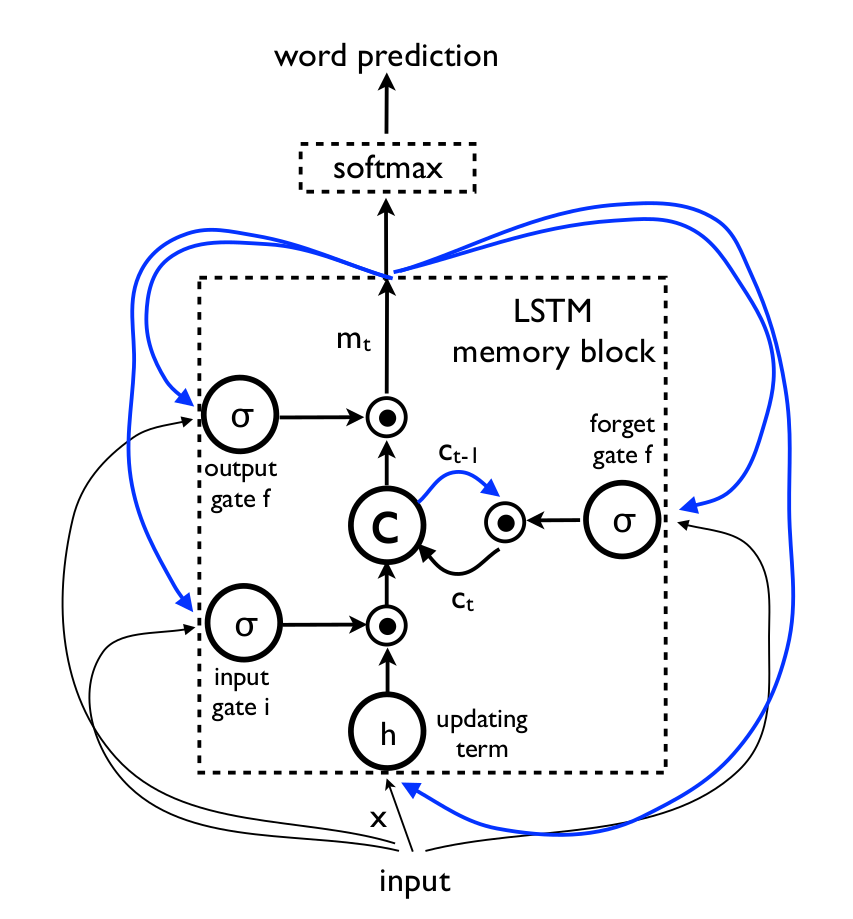
\includegraphics[scale=0.266]{LSTM_unit.png}
					\caption{A single LSTM unit\label{fig6}}
				\end{figure}
				Long Short Term Memory Networks are a type of Recurrent Neural Networks. These networks are based upon recursion, so that variable length inputs can be handled easily and sequential information can be processed with better results. LSTM's are specifically used for making RNNs learn long term patterns since traditional RNNs tend to \textbf{favour short term temporal dynamics}. It can be difficult to train traditional RNNs to learn long-term dynamics, likely due in part to the \textbf{vanishing and exploding gradients problem} that can result from propagating the gradients down through the many layers of the recurrent network, each corresponding to a particular time step\cite{ltms}. LSTMs provide a solution by incorporating memory units that explicitly allow the network to learn when to ``forget'' previous hidden states and when to update hidden states given new information\cite{lstmexecute}.\\
%				Below we list the main equations governing the behaviour of the LSTM networks.\\
%				\begin{align}
%					f_{t} &= \sigma_{g}(W_{f}x_{t} + U_{f}h_{t-1} + b_{f})\\	
%					i_{t} &= \sigma_{g}(W_{i}x_{t} + U_{i}h_{t-1} + b_{i})\\
%					o_{t} &= \sigma_{g}(W_{o}x_{t} + U_{o}h_{t-1} + b_{o})\\
%					c_{t} &= f_{t} \circ c_{t-1} + i_{t} \circ \sigma_{c}(W_{c}x_{t} + U_{c}h_{t-1} + b_{c})\\
%					h_{t} &= o_{t} \circ \sigma_{h}(c_{t})
%				\end{align}
%				The symbol meanings are:\\
%	$\mathbf{x_{t}}$: Input vector\\
%    $\mathbf{h_{t}}$: Output vector\\
%    $\mathbf{c_{t}}$: Cell state vector\\
%    $\mathbf{W}$, $\mathbf{U}$ and $\mathbf{b}$: Parameter matrices and vector\\
%    $\mathbf{f_{t}}$: Forget gate vector. Weight of remembering old information.\\
%    $\mathbf{i_{t}}$: Input gate vector. Weight of acquiring new information.\\
%    $\mathbf{o_{t}}$: Output gate vector. Output candidate\\
%    $\mathbf{\sigma_{g}}$, $\mathbf{\sigma_{c}}$ and $\mathbf{\sigma_{h}}$: Activation functions\\
		
			\subsection{Training Deep Neural Networks}
					\begin{figure}[ht!]
					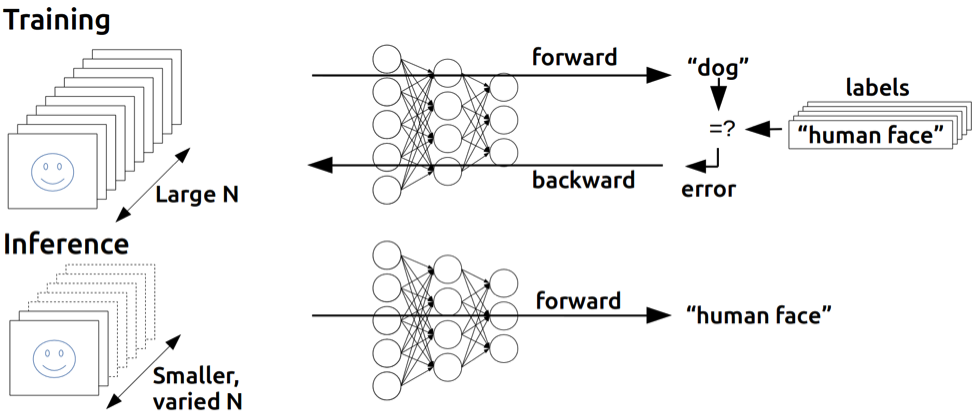
\includegraphics[width=14cm]{training_inference1.png}
					\caption{Training and Inference Processes\label{fig5}}
				\end{figure}
				A Deep Neural Network is at it's core a parameter based function. All of these parameters are  \textbf{trained} automatically from inputs and expected output tuples (training data). The training process revolves around minimizing a particular cost function using methods like \textbf{Stochastic gradient descent}. The input is given to the network in a feed forward fashion and the parameters are modified from the last layer to the first \textbf{(Backpropagation)}. Neural Networks, by design, require huge amounts of training data and take a large time to get trained. For some perspective, most current state of the art image classifiers have $> 100$ million parameters and are trained on more than 1.2 million images. 


			\subsection{Finetuning}
				Fine-tuning a network is a procedure based on the concept of
				\textbf{transfer learning}. We start training a CNN to learn features for a broad domain with a
				classification function targeted at minimizing error in that domain. Then, we
				replace the classification function and \textbf{optimize the network} again to minimize
				error in another, more specific domain. Under this setting, we are transferring
				the features and the parameters of the network from the broad domain to the
				special one.\cite{fineplant} In our project we will need to use the pre-trained image classification models 
				to actually decode individual frames of the video, thus we are planning to \textbf{fine-tune those models
				with respect to the output of our LSTMs}.



	\begin{thebibliography}{1}
	
	  \bibitem{proposal} Subhashini Venugopalan {\em Natural Language Video Description using Deep Recurrent Neural Networks}, 2015.
	
	  \bibitem{s2vt}  Venugopalan, Subhashini and Rohrbach, Marcus and Donahue, Jeff
                    and Mooney, Raymond and Darrell, Trevor and Saenko, Kate {\em Proceedings of the IEEE International Conference on Computer Vision (ICCV)}, 2015
	
	  \bibitem{showandtell} Oriol Vinyals and
               Alexander Toshev and
               Samy Bengio and
               Dumitru Erhan {\em Show and Tell: {A} Neural Image Caption Generator} 2014.

        \bibitem{lstmexecute} Wojciech Zaremba, Ilya Sutskever {\em Learning to Execute} ICLR 2015
         

         \bibitem{temporal}  Li Yao, Atousa Torabi, Kyunghyun Cho, Nicolas Ballas, Christopher Pal, Hugo Larochelle, Aaron Courville {\em Describing Videos by Exploiting Temporal Structure} ICCV 2015
        

         \bibitem{visualqa} Aishwarya Agrawal, Jiasen Lu , Stanislaw Antol,
		Margaret Mitchell, C. Lawrence Zitnick, Dhruv Batra, Devi Parikh {\em VQA: Visual Question Answering} 2016
        

         \bibitem{ltms} Jeff Donahue, Lisa Anne Hendricks, Marcus Rohrbach, Subhashini Venugopalan, Sergio Guadarrama, Kate Saenko, Trevor Darrell {\em Long-term Recurrent Convolutional Networks for Visual Recognition and Description} 2016

         \bibitem{deep} Bengio, Yoshua; LeCun, Yann; Hinton, Geoffrey {\em Deep Learning} 2015

         \bibitem{fineplant} Angie K. Reyes, Juan C. Caicedo and Jorge E. Camargo {\em Fine-tuning Deep Convolutional Networks for
		Plant Recognition} LifeCLEF 2015

         \bibitem{cs231n} Andrej Karpathy {\em 
			CS231n Convolutional Neural Networks for Visual Recognition
		} http://cs231n.github.io/convolutional-networks/

		\bibitem{fullyconnected} Santanu Chaudhury, Anupama Mallik, Hiranmay Ghosh {\em Multimedia Ontology: Representation and Applications
		} 

	\end{thebibliography}
\end{document}
